\documentclass[10pt,draftclsnofoot,onecolumn]{IEEEtran}
\usepackage[letterpaper, portrait, margin=0.75in]{geometry}
%\usepackage[myheadings]{fullpage}
\usepackage{fancyhdr}
\usepackage{lastpage}
\usepackage{graphicx, wrapfig, subcaption, setspace, booktabs}
\usepackage[T1]{fontenc}
\usepackage[font=small, labelfont=bf]{caption}
%\usepackage{fourier}
\usepackage[protrusion=true, expansion=true]{microtype}
\usepackage[english]{babel}
%\usepackage{sectsty}
\usepackage{url, lipsum}
\usepackage{tikz}
\usepackage{listings}
\usepackage{placeins}

\newcommand{\namesigdatehrule}[1]{\par\tikz \draw [blue, densely dotted, ultra thick] (0,0) -- (#1,0);\par}
\newcommand{\namesigdate}[2][5cm]{%
\begin{minipage}{#1}%
    #2 \vspace{0.8cm}\namesigdatehrule{#1}\smallskip
    \small \noindent\textit{Signature}
    \vspace{0.8cm}\namesigdatehrule{#1}\smallskip
    \small \textit{Date}
\end{minipage}
}


\newcommand{\HRule}[1]{\rule{\linewidth}{#1}}
\newcommand*\tick{\textsc{\char13}}
\singlespacing
\setcounter{tocdepth}{5}
\setcounter{secnumdepth}{5}


\begin{document}
%\title{HyRo (Working title)}
%\author{Jason Klindtworth  |  Josh Asher  |   Layne Nolli}
%\date{}
%\maketitle
\begin{titlepage}
	\centering
	{\scshape\LARGE HyRo \par}
	\vspace{1cm}
	{\scshape\Large Jason Klindtworth  |  Josh Asher  |   Layne Nolli\par}
	\vspace{1.5cm}
	{\huge\bfseries CS461\par}
	\vspace{2cm}
	{\huge\bfseries Team 28\par}
	\vspace{2cm}
	{\Large\itshape Fall 2016\par}
	\vspace{4cm}
	{\Large\itshape Fall Term Progress Report\par}
	\vspace{4cm}
	{\large Abstract\par}
	\vspace{1cm}
	We are now in our second term of capstone and this paper documents the first half of that term. There have been fewer struggles this term but still many mysteries. This paper details our failures, hardships and success's. Overall we are were we need to be at and excited about launching this rocket up to 10,000 feet!\par

	\vfill

% Bottom of the page
	{\large \today\par}
\end{titlepage}


\section{Overview of Purpose and Goals}
{\bf Jason, Josh, and Layne all took equal parts in writing these sections before our individual weekly blogs} \par
OSU has for the past 2 years had seniors from MIME and ECE develop a hybrid rocket for their capstone projects. The first years didn't even get off the ground, but through their efforts lasts years team was able to build a hybrid that went 5000 feet. They were able to build a system to collect a large amount of data from on-board sensors, but had no way to easily visualize it. That's why we were invited aboard. This is the first year a CS team has worked on the hybrid rocket team. Our goals are to provide visualization to their data along with providing remote controls (like filling the oxidizer tank) to allow the team to operate the rocket entirely from a safe distance. We have been working closely with our ECE counter parts in this second third of our capstone experience. \par
Last term we had completed our major design documents. This proved challenging on many levels. We had to not only get to know ourselves well, but learn to work well together. Then repeat that same process with a 15 member team. There were a lot of bumps in the road including communication, understanding, and learning. In the long run we all need to develop an entire hybrid rocket, launch it 10000 feet, and visualize the data from the onboard components. \par
This term we have begun our development of our project. Or goals at this point of the progress report our to get it to an alpha stage. For us that means getting the radio transceiver communication working, setting up the user interface with all of its components, and begin to give those components functionality. Then we want to solidify receiving data, visualizing and logging it. Graphics are not our biggest concern at the moment. We want to get our project as far along as possible so we can spend next term smoothing the data flow and looks out. \par
Another big goal for this term is to revise our original design documents. During the course of this progress report we all have taken the time to revise our sections. Not a whole lot of things have change, but there were some major changes. These will be mentioned under the next section. The goal in the long run is to have a set of documentation that professionally describes our system and the road we took to get to the solution. Currently we have speeches and a rough draft of our poster to look forward too. \par
\section{Where We Are Currently and Where we Need to Head}
We have begun development of our user interface and its backend as well as starting work on the communication between the rocket at the ground computer. This communication is going to be done by radio transceivers called XBees. The user interface is at an alpha stage, but we are very comfortable in the amount of progress we have made on it. It has all the buttons that have been requested for the rocket commands. Including the call back functions for the buttons that will send data to the onboard rocket system. This does not yet send data to the XBee, but is one of our current coding problems. We have created classes for drawing the graphs and gauges on our interface. They look fairly ghetto right now, but Jason is going to work on graphics to make them look better. Right now they are draw using the Tkinter canvas drawing functions. We were also successful in implanting the Matplotlib library and using it to draw graphs on the canvas widgets.\par
As far as the user interface backend is concerned we have all the thread and initialization functions necessary to start XBee communication and initialize the user interface. One of the next steps is to code all of the data buffers and log arrays into the program. When this is done we will code in the loading function that will load data into these arrays to display on the screen. We will have not done much work on the data processing yet, but we are close. \par
We received the XBees and a Beagle Bone Black to experiment with. On the traditional computer side we installed the XBee python library and were able to get the computer to talk to its XBee that was connected via USB. We did this by creating a python thread that initializes the serial port and XBee then loops with a callback function to receive transmission. This was successful, we will now code the send function. This was a very exciting accomplishment.\par
There were some major changes that came up this term so far. Mainly we found out that the ECE team will be covering collecting sensor data and controlling electronic components.They will interface with us on the Beagle Bone Black in the system and send us this info. We are responsible for the same communication of commands back to their program. This has saved us a lot of time and we feel we will have time to reach our stretch goal of gps.\par
The rocket currently has finally begun its development stage. A lot of components were not chosen until this week. This has left us and the ECE team really in the dark as far as design goes. Now the ECE team has finalized there stuff and is ready to communicate with us because the ME team has finally decided on the components and dimensions of their rocket. This is a very fun process to watch, especially test fires. \par
For the rest of the term we plan on getting our document signed and getting the system into full working beta. There are some unknowns still like the tank pressure, but we want to be far enough along that adding such a component will be easy. First though we will make sure all the currently selected requirements our met by the end of the term. We would like to spend next term refining our product. \par

\section{Major Problems And Solutions}
This term has proven to be a lot less problem prone. Our first term consisted of major communication problems that we have through persistence dealt with. The first half of the second term has a new set of problems. We began developing our project and the major road block in that situation has been time. It has been difficult to get together more than once a week and work together on the program. To deal with this problem we have used our meetings to discuss major decisions in the program and plan out ways to approach individual aspects of the program. This has proven very effective and we have worked well on our individual components. We feel comfortable that we will be at full functional beta by the end of the term. \par
Another major problem that has persisted since last term is the lack of the other teams components being far enough along to really determine aspects that we have been uncertain about. The ECE team has been working very hard on their components, but they too have been waiting for the ME team to make decisions. That has not been possible until this term. The ME team is now far enough to start making appropriate design decisions. These decisions will trickle down to us and we will be better able to define certain aspect of our system. This problem has made a lot of our work challenging. We have not been able to answer certain questions about what all will be in our software at the end of the year.We have conquered this so far by designing a system that will work with what every data they present us. We have a rough idea of the needs of our client and now they are finally starting to come to fruit. This is always a fun and exciting part on engineering and we knew the process would be like this. As the rocket design moves further along all teams are really getting excited about this launch. So much so that if we do well this year they will use it as a base line for other hybrid rocket projects from other schools. \par
A common issue that will persist through the entire course of this project is time. We are all taking senior level classes and it is hard to squeeze any time in for anything. Two of us have kids and we all know how much time they take up. We attack this problem by having open communication. We have learned how we best communicate with each other and we email almost daily. This keeps us all on the same page and we know when we have to put extra work in to accomplish our tasks It has been especially weird since we have not had that much class time. We have had to learn to work around this and keep in close contact.\par
One of our major software related problems is and will be the lack of data. We have some data from last year, but it is hard to fake launching a rocket. Measuring data from a avionics bay that is stationary will not give us an accurate representation of what it is going to look like live. There are two major approaches we are taking to conquer this issue. First we are designing our problem to load old data and are going to run last years data over and over again to test our user interface. Second we are trying to come up with creative ways to make the sensors pick up data. We need to be able to drop our bay from high up. So we plan to find a very tall building and make a mock avionics system. This seems possible as everyone has bought multiple copiers of all major components. We do not want to go into the launch blind, so if we have to jump out of an airplane we will do so. \par

\section{Interesting Piece of Code}
Here is our current Xbee class, it is an extension of the python threading class that initializes and listens to an XBee radio transceiver. This is pretty cool, that means you can hook up another transceiver to what every you want and communicate with it. \par

\begin{lstlisting}
class xb_rcv_thread(threading.Thread):
    def __init__(self, threadID, name, counter, q, port):
        threading.Thread.__init__(self)
        self.threadID = threadID
        self.name = name
        self.counter = counter
        self.port = port
        self.serial = self.init()
        self.xbee = XBee(self.serial, callback=self.processMessage)
        self.q = q

    def run(self):
        print("Starting " + self.name)
        #self.xbee.tx(dest_addr=b'\x00\x01', data=b'Hello World')
        self.listen()
        print("Exiting " + self.name)

    def init(self):
        try:
            # Open serial port
            print("opening comm")
            #ser = serial.Serial('COM4', 9600)
            return serial.Serial(self.port, 9600)

            # Send the string 'Hello World' to the module with MY set to 1
            #xbee.tx(dest_addr=b'\x00\x01', data=b'Hello World')
       
        except KeyboardInterrupt:
            pass

    def end(self):
        self.xbee.halt()
        self.ser.close()

    def listen(self):
        while 1:
            time.sleep(0.001)

    def processMessage(self, data):
        #print(data["rf_data"])
        self.q.put(item=data["rf_data"], block=False)

\end{lstlisting}
\pagebreak

\section{Current Screen Shot}
Please forgive us, this is alpha, but here is what the GUI looks like so far. No graphics have been developed yet to make it look pretty. \par

\begin{figure}[!ht]
  \caption{Current shot of alpha graphical user interface.}
  \centering
	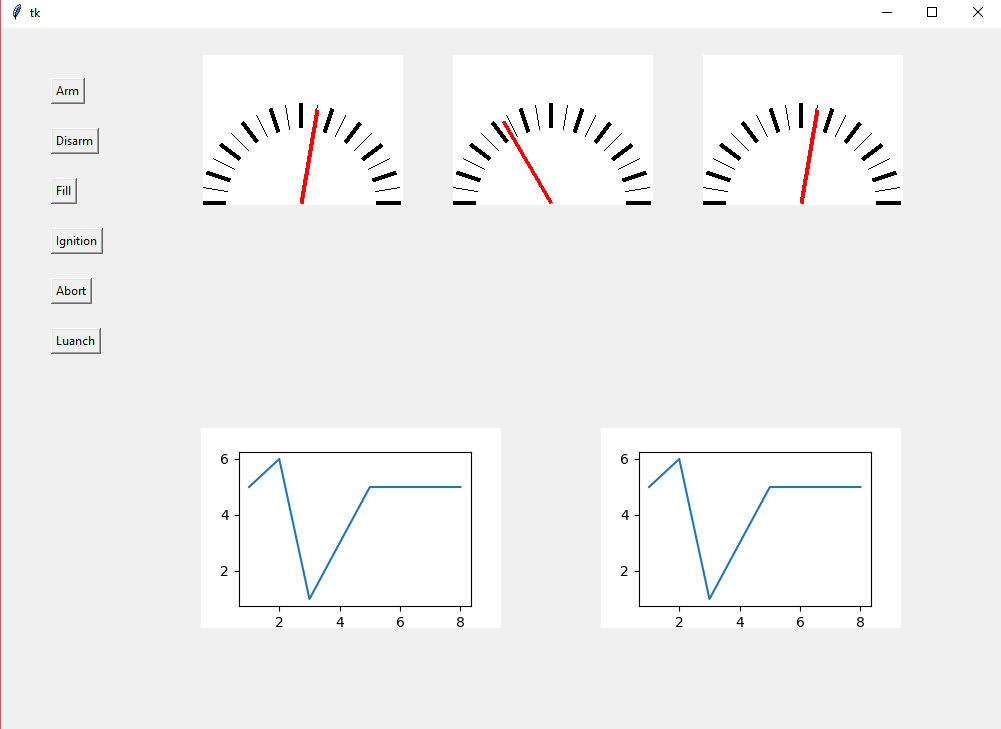
\includegraphics[scale=.85]{AlphaGui}
\end{figure}
\FloatBarrier

\section{Week by Week Recap}
The following is a week by week recap from each team member up to week 5 of winter term.  \par

\subsection{Week 1}
\subsubsection{Josh Asher}
 I am excited to be back from winter break. Looking for to the major development portion of our project. Just remembered we all need to sign up for the AIAA, totally forgot about that. We were able to get a few things done over the break. Our development environment is set-up and working. We for the moment are trying out the Visual Studio python extension and it is working great so far. We were able to get a few things up on our GUI, this will be coming along faster now that we are back focused on school. Next week we plan to get the layout of the GUI finalized and work on the graphing utilities. I will be ordering a couple pieces we don't have so at some point we can get to work on the serial communication part of this project. Should be a great term! \par

\subsubsection{Jason Klindtworth} 
We did not get a whole lot done over the break. We were hoping to get together a few times but it just did not work out with all of the traveling and icy conditions that ended up happening. We were able to independently get a bit worked on for our project however. We got a few working buttons and things up and working on a functional GUI. We will continue to tweak and change the layout until we find a design that we are both happy with, and will work for the project. Now that we are back in school and meeting regularly we should be able to ramp up the development progress in the next few weeks and are hoping to be most of the way done with the project by the end of this term. \par

\subsubsection{Layne Nolli}
We didn't get any work opportunities over the break but once the start-of-term turmoil has settled I have full confidence in our team being able to get down to business on the project. Need to sign up for AIAA. Goals for the term are to be mostly done by the time spring rolls around to leave lots of room for last minute adjustments. \par

\subsection{Week 2}

\subsubsection{Josh Asher}
This week we arranged meetings for both the TA and the rocket group meetings. So starting next week that should all be on schedule. We are planning on meeting on the weekends hopefully as a group. We think the initial part of out project including the GUI and the traditional computer side of things will go easy and be quick. We are kinda concerned about the progress of the ECE team, we haven't heard from them. During the rocket meeting next week we should hear from them. All our data we will be visualizing is coming from there setup so we are working the other direction towards that. Hopefully things are going well for them. I am purchasing a beagle bone for testing and later fro fun so we can work on the USB and radio communication. \par

\subsubsection{Jason Klindtworth}
We are sort of in a waiting pattern at the moment. We are waiting for the ECE members of our group to lock down some of the hardware design so we know which direction we need to take the programming part of our project. Josh is hopefully going to get his hands on a beagle-bone micro-controller this week so we can start running some tests and see what we have as far as capabilities with the hardware. We also finalized our meeting times with our new TA and had our first meeting this week. We are still in the process of figuring out when our meeting times will be for the HyRo group as a whole, but hopefully those well start pretty soon as well.  \par

\subsubsection{Layne Nolli}
Set up meeting times with TA, Rocketry group meetings, and are looking to finalize a meet time for the CS branch of the Rocketry group still. Currently as a team we are waiting for the ECE teams current hardware status so we can set up some target goals and begin furthering the progress we have on the CS side of things. \par

\subsection{Week 3}

\subsubsection{Josh Asher}
 We had a weird week. No class and TA had to cancel on us. We did however have our first Hybrid meeting of the term and Nancy was actually there. Which was awesome. The ECE team is coming along and we should be meeting up with them in the project here in the next few weeks. We have a slack page for the entire rocket team. Everyone is very excited and so are we about this project. The GUI hasn't made it to much further, but we are meeting all together on Sunday to do some work on it. The beagle bone and radio transceivers should be in on Monday so we can start to work on the USB communication. Hopefully python is nice to us and that is rather easy. Once the GUI is prettier we will post some picture of it and the BBB. \par

\subsubsection{Jason Klindtworth}
 Our TA canceled our weekly meeting this week at the last minute, so we did not have a chance to meet up. We did get our code posted to github (the start of it) and we did some layout and planning for the final design. We are planning on meeting up as a group at my house on Sunday so we can get some work done. We should be able to make good progress during that time. A lot of the work we are still waiting on the ECE crew to make final decisions about their portion of the design before we are able to move forward, but hopefully that will not take too much longer. \par

\subsubsection{Layne Noll}
No Class this week and we had a surprise cancellation from the TA as well. We were able to touch base with the ME/EE portions of our rocket design team during the first weekly meet up for this term however. Things seem to be going well on their end and we (the CS guys) are in a bit of a holding pattern until the ECE guys make a couple component decisions. Josh and Jason have made a little headway on the python GUI and I intend on tagging in for some hands-on work on that later this coming week.  \par\

\subsection{Week4}
\subsubsection{Josh Asher}
 Everyone got a grip on the development environment this week. We are going to make some design changes as we have ran into better ideas while coding. These will be updated in the design dock. The BBB and the Xbee transceivers came in this week, but we haven't had time to play with them yet. This will be one of the major goals for next week. We need to make sure we establish and come up with good routines to talk back and forth with the Xbees. The GUI came on a little bit and is defiantly approaching and alpha stage. Our meeting with the TA went well. We are waiting on the approaching assignments with anticipation, but we have plenty of changes and progress to report on. We plan on working on the code more next week and having a meeting with the ECE team to try and nail out a protocol. \par

\subsubsection{Jason Klindtworth}
The group meeting on Sunday was very successful. We were able to get out development environment set up and working and also made quite a bit of progress on the layout of the UI. The graphs and buttons are going to need some additional work but so far they are looking good. We had class this week and got some more information about the upcoming assignments for the class and we are planning on getting together again this weekend to work on the progress report video and make more progress on the UI. We still cannot work on the backend of our program yet without further progress from the ECE team, but we will keep in touch with them and hopefully be able to get started on it soon. \par

\subsubsection{Layne Nolli}
This week we discussed design idea changes and got a good handle on what the cross disciplinary teams were up to. Josh picked up the hardware we are going to use for testing and development, so huge props to him. Development on alpha is getting going, we have a basic UI and placeholder data in place. \par

\subsection{Week 5}
\subsubsection{Josh Asher}
We have made significant progress this week on our code. We have successfully got the BBB connected to its XBee and the other XBee connected to a laptop. This was tricky at first, we had to find the correct python library to use and there was some issues when initially trying to setup the XBee's. We learned by using the Digi program XTCU we could modify the XBee's addresses and set there mode. At first we couldn't get the XBee's to talk and when we sent a message the whole program would crash. This is because we did not have the transceivers in API mode. This is the only mode our python library would function in! After that was figured out we did some test sends and receives. In our program we are now developing a thread that will run parallel to the main program that is in charge of sending and receiving message between the computer and beagle bone. When it receives a message it will place into a queue that will be processed by the main thread. We have got a deadline for our progress report and document revisions so we are setting up meetings to hammer these out. We are going to do our video on Sunday at Jason's. From here out we first plan to get our written assignments done then start coding the data structures and get data feeding into the gauges and graphs. \par

\subsubsection{Jason Klindtworth}
This week we started working on our revisions for the upcoming assignments. We also worked on finalizing our development environment and got to work on some code, we got the Xbee radio transceiver connected and talking with our software, which is a major step. We were pretty busy as a group this week and weren't able to get a whole lot done. But we are planning another meeting on Sunday to work on the video presentation and hammer out the detail of our revisions for the documents. \par

\subsubsection{Layne Nolli}
Learning about the hardware is going well. Josh got us caught up on the hardware he picked up for testing and we had a good opportunity during our group meeting to catch up on where the code is at and what needs to be worked on. A lot of other class work and midterms are falling due around this time so the group and the cross disciplinary groups have had their hands quite full. Going to be dealing with all of this paper revision and the presentation this wekk. Looking forward to making some more headway in the coming week on our code development. \par

\section{Retrospective}
\begin{tabular}{ |p{0.3\linewidth}|p{0.3\linewidth}|p{0.3\linewidth}| }
\hline
\multicolumn{3}{|c|}{Retrospective} \\
\hline
    Positives & Deltas & Actions \\
\hline
    We have an awesome client that is very easy to deal with. This is a repeat, but we feel really lucky. She is super nice and helpful not only on the project, but with resources to jobs. & Need to meet more on the weekends. This is also a repeat, but we are constantly dealing with it. & We try and have a meeting in the middle at Jason's house on Sundays. \\
\hline
    The rocket is starting to actually be design by the MEs. & Have to meet with Nancy more.& Dr. squires is starting to attend the meetings and we are making efforts to keep her informed. \\
\hline
Our team continues to get along very well. & We need to finish the data structures to hold our data. & We have begun to develop this and should be pretty much done in the next coupe of meetings. \\
\hline
The ECE team is far in their project and ready to communicate with our system. & Some components on the rocket are still undecided. & We will pay close attention to the ME's and their designs and as soon as we know a component is to be added we will add that component to our system.\\
\hline
Our GUI is well into the alpha stage and will be ready for beta by the end of the term. & We are going to have a hard time testing the system with accurate data. & We will develop testing procedures to generate live data. This could be difficult, but is essential to our project. \\
\hline
We should have time for a couple stretch goals. & We need to reserve time to connect our system with the ECE team. & We have begun to plan these meetings. They should start before the end of the term. \\
\hline
Our documents have been easy to revise. & We need to develope better graphics. Our program looks dated currently. & Jason has good software for graphics and is experienced in the subject. He has begun designing elements of the graphical user interface. \\
\hline

\end{tabular}
\end{document}